\section{Week 5}
\textbf{$\mathcal{Z}$-plane stability: z is real}
\begin{figure}[H]
    \centering
    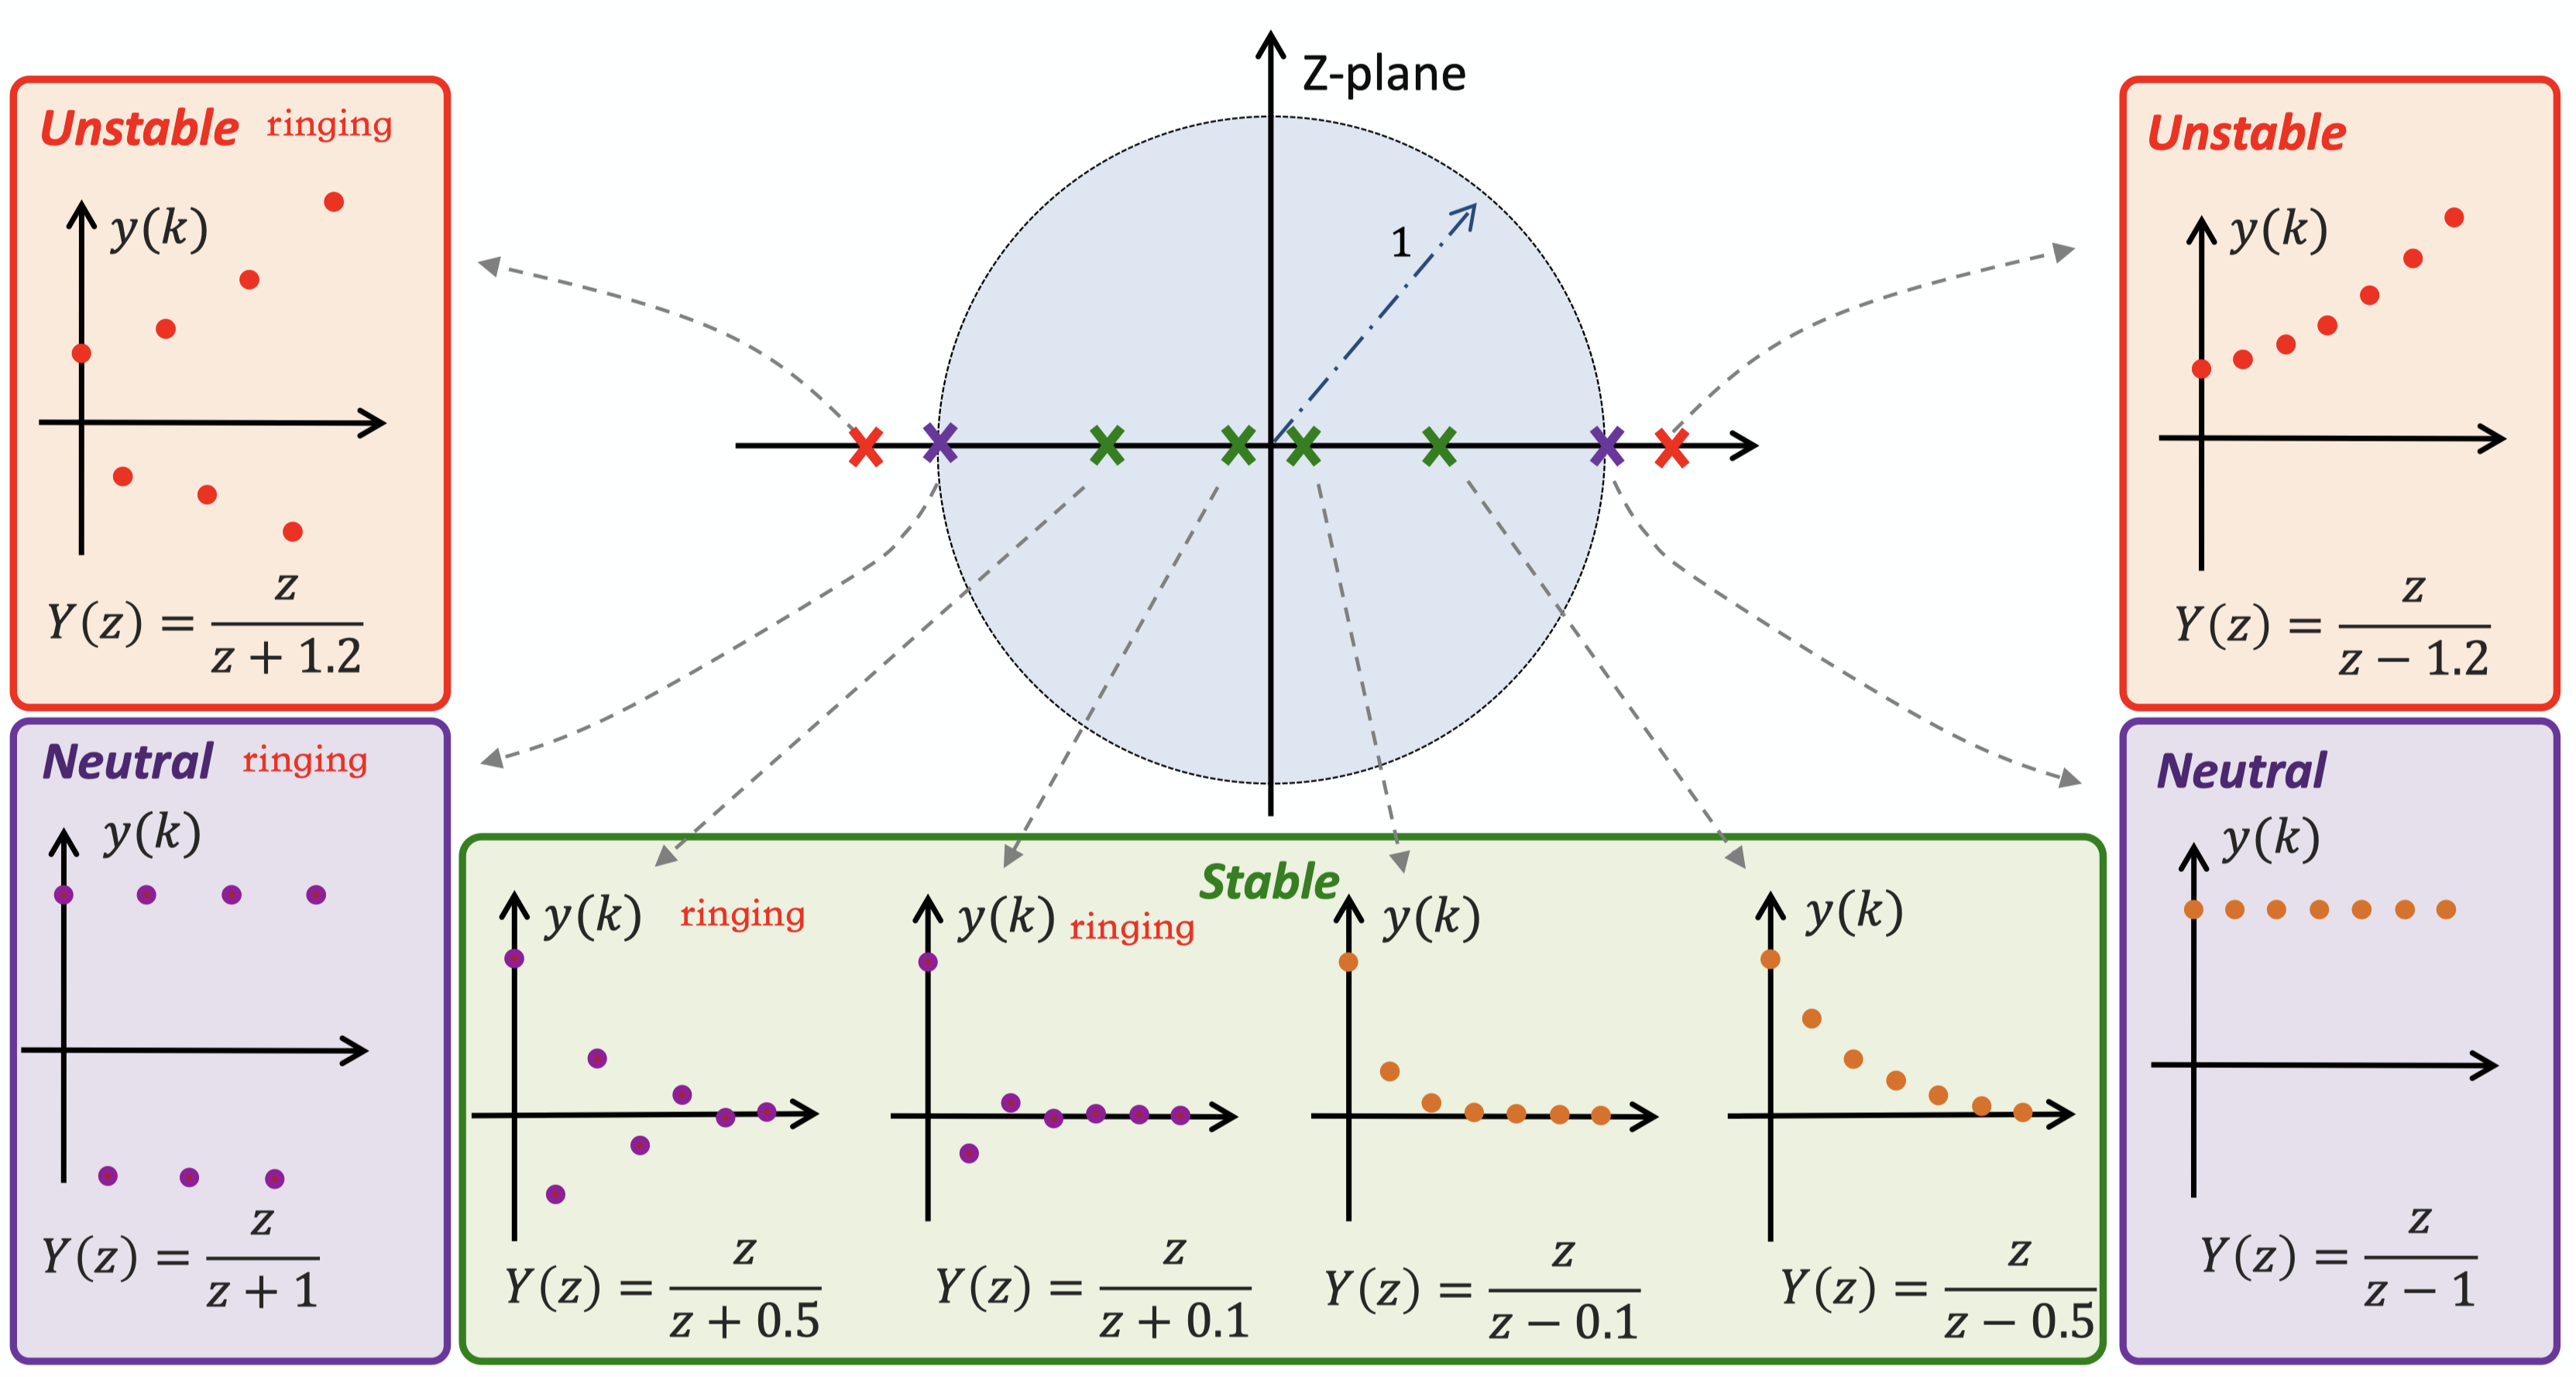
\includegraphics[width=0.5\textwidth]{images/z_plane_stability.png}
\end{figure}

\begin{table}[h]
\begin{adjustbox}{max width=\textwidth}
\begin{tabular}{|c|p{0.2\textwidth}|c|c|}
\hline
\textbf{$z=a$} & \textbf{transient response} & \textbf{stability} & \textbf{ringing?} \\\hline
$a> 1$ & transient term will grow & unstable & No \\\hline
$a = 1$ & transient term will remain constant & neutral & No \\\hline
$0<a<1$ & transient term will die down & stable & No \\\hline
$a=0$ & transient term will disappear in one sampling interval & stable & No \\\hline
$-1<a<0$ & transient term will disappear & stable & Yes \\\hline
$a = -1$ & transient term will ring with constant amplitude & neutral & Yes \\\hline
$a < -1$ & transient term will ring and grow & unstable & Yes \\\hline
\end{tabular}
\end{adjustbox}
\end{table}
\clearpage

\textbf{$\mathcal{Z}$-plane stability: z is complex}
\begin{table}[h]
\begin{adjustbox}{max width=\textwidth}
\begin{tabular}{|c|c|c|}
\hline
\textbf{$z=p\pm jq = re^{\pm j\theta}$} & \textbf{$Cr^k \cos(k\theta + \phi)$} & \textbf{stability} \\\hline
$r\ge 1$ & oscillatory, grow to $\infty$ & unstable \\\hline
$r=1$ & oscillatory, stay steady & neutral $a=-1$ \\\hline
$0<r<1$ & oscillatory, disappear as $t\to\infty$ & stable  \\\hline
$r=0$ & disappear in one sample interval & stable \\\hline
\end{tabular}
\end{adjustbox}
\end{table}

\textbf{Important Difference between s- and z-plane:} double poles on the unit circle (a ramp) is not stable!

\textbf{\large S-plane and z-plane mapping}
\begin{equation*}
    s=\sigma + j\omega \xrightarrow{z=e^{Ts}} z = e^{Ts}e^{j(T\omega + 2 \pi)}
\end{equation*}
\begin{align*}
    s &= s+ j \omega_d \begin{cases}
    \sigma = \frac{\ln(r)}{T} \\
    \omega_d = \frac{\theta}{T}
    \end{cases} \\
    C_0 &= -\frac{\sigma}{\omega} = - \frac{\ln(r)}{\theta} = -\sqrt{\frac{\zeta}{1-\zeta^2}} 
\end{align*}
\begin{figure}[H]
    \centering
    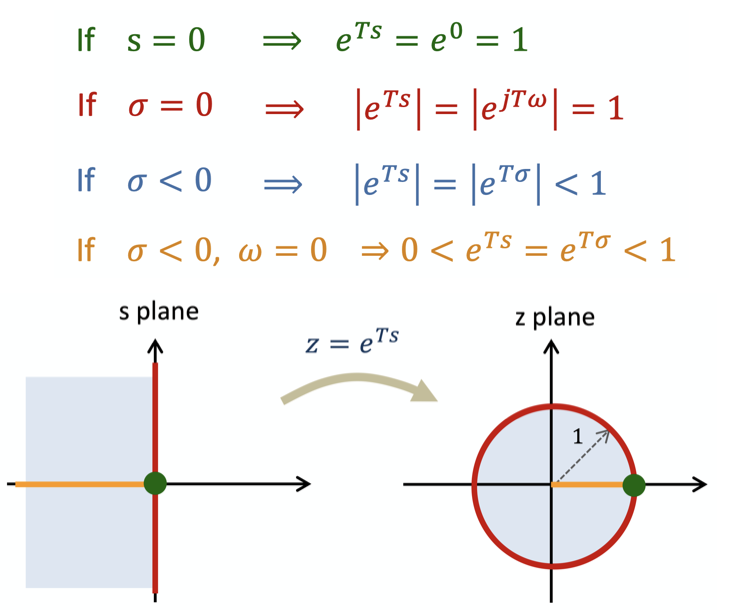
\includegraphics[width=0.5\textwidth]{images/s_z_mapping.png}
\end{figure}

\textbf{\large Dominant poles in z-plane}: 

the poles closer to the unit circle are the dominant/slowest poles.

\textbf{\large Steady state gains}
\begin{itemize}
    \item \textbf{DC Gain} = $\lim_{z\to 1} G(z)$ 
    \item \textbf{Inst. Gain} = $\lim_{z\to \infty} G(z)$
\end{itemize}

\textbf{\large Discrete State Space}
\begin{equation*}
    \begin{cases}
     \dot{x}(t) = \bm{A}x(t) + \bm{B}u(t) \\
     y(t) = \bm{C}x(t)+\bm{D} u(t)
    \end{cases}, \; \begin{cases}
     x(k+1) = \bm{G}x(k) + \bm{H}u(k) \\
     y(kT) = \bm{C}x(kT) + \bm{D}u(kT)
    \end{cases}
\end{equation*}
\begin{align*}
    \text{where } \bm{G} &= e^{\bm{A}T} \\
    \bm{H} &= \int_{0}^{T}\left(e^{\bm{A}\lambda} d\lambda\right) \bm{B} \\
    &= \bm{A}^{-1} (e^{\bm{A}T}- \bm{I})\bm{B}
\end{align*}